\documentclass[]{article}\usepackage[]{graphicx}\usepackage[]{color}
%% maxwidth is the original width if it is less than linewidth
%% otherwise use linewidth (to make sure the graphics do not exceed the margin)
\makeatletter
\def\maxwidth{ %
  \ifdim\Gin@nat@width>\linewidth
    \linewidth
  \else
    \Gin@nat@width
  \fi
}
\makeatother

\definecolor{fgcolor}{rgb}{0.345, 0.345, 0.345}
\newcommand{\hlnum}[1]{\textcolor[rgb]{0.686,0.059,0.569}{#1}}%
\newcommand{\hlstr}[1]{\textcolor[rgb]{0.192,0.494,0.8}{#1}}%
\newcommand{\hlcom}[1]{\textcolor[rgb]{0.678,0.584,0.686}{\textit{#1}}}%
\newcommand{\hlopt}[1]{\textcolor[rgb]{0,0,0}{#1}}%
\newcommand{\hlstd}[1]{\textcolor[rgb]{0.345,0.345,0.345}{#1}}%
\newcommand{\hlkwa}[1]{\textcolor[rgb]{0.161,0.373,0.58}{\textbf{#1}}}%
\newcommand{\hlkwb}[1]{\textcolor[rgb]{0.69,0.353,0.396}{#1}}%
\newcommand{\hlkwc}[1]{\textcolor[rgb]{0.333,0.667,0.333}{#1}}%
\newcommand{\hlkwd}[1]{\textcolor[rgb]{0.737,0.353,0.396}{\textbf{#1}}}%

\usepackage{framed}
\makeatletter
\newenvironment{kframe}{%
 \def\at@end@of@kframe{}%
 \ifinner\ifhmode%
  \def\at@end@of@kframe{\end{minipage}}%
  \begin{minipage}{\columnwidth}%
 \fi\fi%
 \def\FrameCommand##1{\hskip\@totalleftmargin \hskip-\fboxsep
 \colorbox{shadecolor}{##1}\hskip-\fboxsep
     % There is no \\@totalrightmargin, so:
     \hskip-\linewidth \hskip-\@totalleftmargin \hskip\columnwidth}%
 \MakeFramed {\advance\hsize-\width
   \@totalleftmargin\z@ \linewidth\hsize
   \@setminipage}}%
 {\par\unskip\endMakeFramed%
 \at@end@of@kframe}
\makeatother

\definecolor{shadecolor}{rgb}{.97, .97, .97}
\definecolor{messagecolor}{rgb}{0, 0, 0}
\definecolor{warningcolor}{rgb}{1, 0, 1}
\definecolor{errorcolor}{rgb}{1, 0, 0}
\newenvironment{knitrout}{}{} % an empty environment to be redefined in TeX

\usepackage{alltt}
\usepackage{fontspec}
\usepackage{graphicx}
\usepackage{float}
\usepackage[left=1.27cm,top=1.27cm,right=1.27cm,bottom=1.27cm]{geometry}
\usepackage{pbox}
\setmainfont{Cambria}

% latexmk -pdf -pdflatex="xelatex -interaction=batchmode" -use-make -quiet tmle.tex

% If you use Biber, then you will have to compile and recompile.
% But Biber seems to be the preferred choice.
\usepackage[backend=biber,sorting=none,style=numeric-comp]{biblatex} 

\addbibresource{tmle.bib} % Critical that you put .bib in here!
\IfFileExists{upquote.sty}{\usepackage{upquote}}{}

\begin{document}
\title{Hospital readmissions and targeted maximum likelihood estimation}
\author{Aman Verma}
\date{\today}
% \maketitle


\section{Introduction}
% Why is this question important to answer?
It is particularly important to accurately estimate the independent effect of hospital treatment on readmission because it is being used to financially penalize hospitals.

% Why it doesn't matter what a preventable readmission is if you have properly stated the counterfactual.
Several readmission risk models have been criticized on the basis that they failed to distinguish preventable readmissions from readmissions due to chance alone. Despite evidence that clincians cannot reliably distinguish preventable and non-preventable readmissions even when given full access to the patient and relevant data, pairs of diagnosis codes have been developed that are "potentially preventable".

% How does this relate to the counterfactual statement?
The counterfactual model clarifies the study question: What is the difference in the proportion with an emergency readmission within 30 days if all patients had attended Hospital A vs Hospital B? The notion of a "preventable" readmission is implicit; if a patient would have been readmitted if treated at another hospital, then the readmission was preventable. 

Since we cannot directly observe the desired proportions, we estimate it by attempting to recreate exchangeability (control for confounding) among the populations that visited different hospitals.

% How do studies typically control for confounding?

% Why is that problematic?

% How can we resolve this?
% TMLE - but because it allows us to include the confounders, but only in so far as they are important to our study question - how much do they confound the relationship between hospitals and redmission.
% For hundreds of covariates, parameteric methods can sometimes be slow and computationally intractable.
% We use techniques borrowed from machine learning. 
% We can use the power of some non-parametric techniques, that are typically difficult to use for inference, to improve our inference through TMLE.

% What is the clear study question?


\section{Methods}

\subsection{Data}
% What does our cohort look like?

\subsubsection{Cohort selection}
We used a cohort extracted from a Canadian provincial (Quebec) administrative database of hospitalizations, obtained from the \emph{Régie de l'assurance maladie du Québec} (RAMQ). We enrolled patients into this cohort on the month that two conditions were satisfied: 1) they had at least one diagnosis of a respiratory illness (the exact list of respiratory International Classification of Diseases, 9th Revision [ICD-9] codes is given in the Appendix) between January 1st, 1996 and March 31, 2006 (the study period), while living in the 2006 census metropolitan area of Montreal, and 2) were at least 65 years of age. We used this cohort because it represents the majority of 65-year olds who were hospitalized in the region during the study period. 

From among this cohort, we selected hospital discharges for those who had accrued at least one continuous year in the cohort preceding the time of admission. We restricted our data to only the discharges from the twenty hospitals with the most discharges of patients 65 years or older within the study period; the twenty hospitals accounted for 75\% of all such discharges.  We only selected hospital discharges which resulted from hospital stays of at least one day. Therefore, the earliest possible hospital discharge was January 2, 1997.

\subsubsection{Hospital readmissions}
The unit of analysis in all models was the hospital discharge; a person could be discharged multiple times. A hospital readmission was defined as an emergency hospital admission to any Quebec hospital in the 30 days following a discharge.  A person who died or had a non-emergency readmission in the 30 days following discharge was considered not readmitted.

\subsubsection{Disease types}
From among the identified hospital discharges, we selected only those with one of three high-volume admission diagnoses with high rates of hospital readmissions: pneumonia, acute myocardial infarction (AMI), and heart failure, the three initial conditions selected by the Centers for Medicare and Medicaid Services (CMS) to implement the Hospital Readmissions Reduction Program mandated by the Affordable Care Act. We identified each of the admission diagnoses using ICD-9 codes; for pneumonia we used codes ranging from 480-487, for heart failure we used all 428 codes, and for AMI we used all 410 codes. The following methods were applied individually to all three disease subsets. 


% Should I talk about the anonymization of hospitals?

% We had confounders.
\subsection{Confounders}
For each hospital discharge, we colllected variables that measured states at the time of admission, or events that occurred prior to the hospital admission, and which may confound the relationship between hospital care and readmission. We used the demographic characteristics (age at time of admission (years), sex, birth year-month), the number of previous readmissions (within the study period), the admission diagnosis (as measured by the specific ICD-9 code). We also included the day of week of discharge, which has been previously shown to have an association with readmissions, and the month of discharge, because we hypothesized that readmission risk would vary by seasons in Montreal.

% What about the census tract of residence?
Additionally, for each discharge, we collected the Quebec hospital diagnoses, Quebec hospital procedures, and drugs dispensed outside of the hospital but inside Quebec, in the year preceding the admission. The hospital procedures were recorded in the Canadian Classification of Diagnostic, Therapeutic, and Surgical Procedures (CCP) system. Hospital diagnostic codes were coded using the ICD-9 system. Finally, drugs which were prescribed and dispensed outside the hospital, and were being taken on the day of admission were also recorded for each patient in the \emph{code commune} system, which categorizes drugs based on the chemical compound. To ease computation, before fitting any model, we removed any diagnosis, procedure or drug that occurred less than 30 times among all discharges. We chose 30 because it appeared to be a natural breakpoint; if the number of variables included is a function $f$ of the threshold, then the first derivative of $f$ dropped at 30 for all three disease categories.

\subsection{Descriptive analysis}

\subsubsection{Choropleth}
We believed that census tract of residence would strongly affect the probability of admission to the hospital nearest that census tract. We plotted choropleths of the rate of attendance at the twenty hospitals by census tract. The numerator was the number of live discharges at the hospital, and the denominator was the number of person-years accumulated in that census tract of residence by cohort members when their admissions would have been eligible (after the first continuous year within the cohort).

\subsection{Models}
\subsubsection{Model $g$ - probability of exposure}
% We built a model G
We developed a multinomial model $g$ that predicted the probability of attending each of the twenty hospitals (the exposure) as a function of all the confounders. To fit $g$ we used a random forest, a non-parametric model based on decision trees \cite{breiman_random_2001}. 

% Explain random forest a bit better?
Our trees were decision stumps; we only used one splitting node at in each tree. We arbitrarily chose to grow 1200 trees (decision stumps), and then measured the accuracy as a function of the numer of trees to ensure that growing further trees would be unlikely to significantly improve accuracy. When measuring the accuracy for each discharge, we only used trees for which the discharge was "out-of-bag", that is, we only used trees for which the bootstrap replicate did not include the discharge.

% We calibrated it based on the weights of the hospital. It was multinomial in that we predicted 20 hospitals. We measured the calibration, similarly only using out-of-bag discharges. We investigated the top 10 variables most important variables, as measured by the Gini coefficient. 
 
% How the Gini coefficient works.
% Make it clear that you didn't invent this.
To assess the importance of the variables in predicting which hospital a patient will choose, for each tree, we calculate the increase in homogeneity of classes between the root of the tree and the leaves. To measure the homogeneity of classes, we repurpose a metric that is typically used to measure equality (homogeneity) of income, the Gini coefficient \cite{gini_variabilita_1912}. The homogeneity is defined as the sum of squared proportions in each class (hospital), with a maximum of 1 (all discharges at the same hospital) and a minimum of 1/20 (the discharges were evenly divided between the 20 hospitals). If the patients within the leaves of the tree made relatively homogeneous hospital choices, this variable predicts hospital choice well.

% How we weighted -- still haven't put in how it was the *Gini* that was weighted.
Because the model was used solely to estimate the \emph{probability} of admission to to specific hospitals (and not to predict exactly which hospital was attended), we configured the model to favour calibration over discrimination: we weighted each of the twenty predicted hospitals by the inverse of the proportion of discharges at that hospital. We multiplied each proportion used to calculate the Gini coefficient by this weight.

Random forest traditionally classifies each item by majority vote; we converted this into a probability by taking the proportion of votes for each hospital (using only out-of-bag trees for each discharge).
% Why did we choose random forest?

\subsubsection{\(Q\) model - probability of outcome}
% We built a model Q
% We built another random forest model, very similar to the model for G, except that instead of predicting the choice of hospital, we predicted 30-day readmission. We also included a set of 19 indicator variables (or was it twenty?) for the hospital. This was also calibrated based on the inverse of the proportion of those readmitted.
For the  \(Q\) model, we developed another random forest model, very similar to the \(g\) model, except that instead of predicting the choice of hospital, we directly predicted 30-day readmission. We also included a set of 19 indicator variables for the hospital attended. We also calibrated this model based on the inverse of the proportion of those readmitted.

We also fit a regularized logistic regression model for \(Q\), using cyclical coordinate descent to estimate the parameters efficiently in our sparse but large matrix. We penalized the likelihood by the \(\ell_2\) norm, that is, the sum of the squares of the normalized regression parameters. The scale of the penalty was determined by the parameter λ. We optimized the selection of the penalty scale for the best partial likelihood using a nested a 10-fold cross-validation. Within each fold we assessed 100 λ-values spaced evenly between max(λ)×10-4 and max(λ), where max(λ) was the smallest λ-value that would result in a model with no non-zero coefficients.

\subsubsection{Variable importance}
% What is the ref for the Gini coefficient?
For each tree, we calculated the decrease in Gini homogeneity when comparing the split nodes of the tree to the root. 
The Gini impurity at any node is, for all out-of-bag discharges.

% To calculate the Gini impurity..
For each hospital, the proportion of patients that chose this hospital $p_h$, multiplied by the probability of guessing that this patient would choose this hospital based on the distribution of patients $1-p_h$. Summed over all hospitals, this is the Gini impurity. Gini impurity is 1 when all patients chose the same hospital.

Gini is defined as "inequity" when used in describing a society's distribution of income, or a measure of "node impurity" in tree-based classification. A low Gini (i.e. higher decrease in Gini) means that a particular predictor variable plays a greater role in partitioning the data into the defined classes. 


\subsubsection{Model Q* - updated targeted maximum likelihood estimation}

% We updated for Q*
To avoid convergence problems for this one parameter model, we fit the parameter using a quasi-Newton method simultaneously discovered by Broyden\cite{broyden_convergence_1970}, Fletcher\cite{fletcher_new_1970}, Goldfarb\cite{goldfarb_family_1970} and Shanno\cite{shanno_conditioning_1970} (BFGS).


\subsection{Software}
We implemented our models using the R statistical package (version 3.1.0) \cite{team_r:_2014}. We implemented the random forest using the "bigrf" package (version 0.1.9) \cite{lim_bigrf:_2014}. We implemented the GLM fitting using coordinate descent using the "glmnet" package (version 1.9.5) \cite{friedman_regularization_2010}. We plotted our figures using the "ggplot2" package (version 1.0.0) \cite{wickham_ggplot2:_2009}.


\section{Results}
% A pretty map for pretty much no reason. It shows that indeed, certain hospitals attract the residents around them, and that this does not vary by disease.
\begin{figure}[H]
    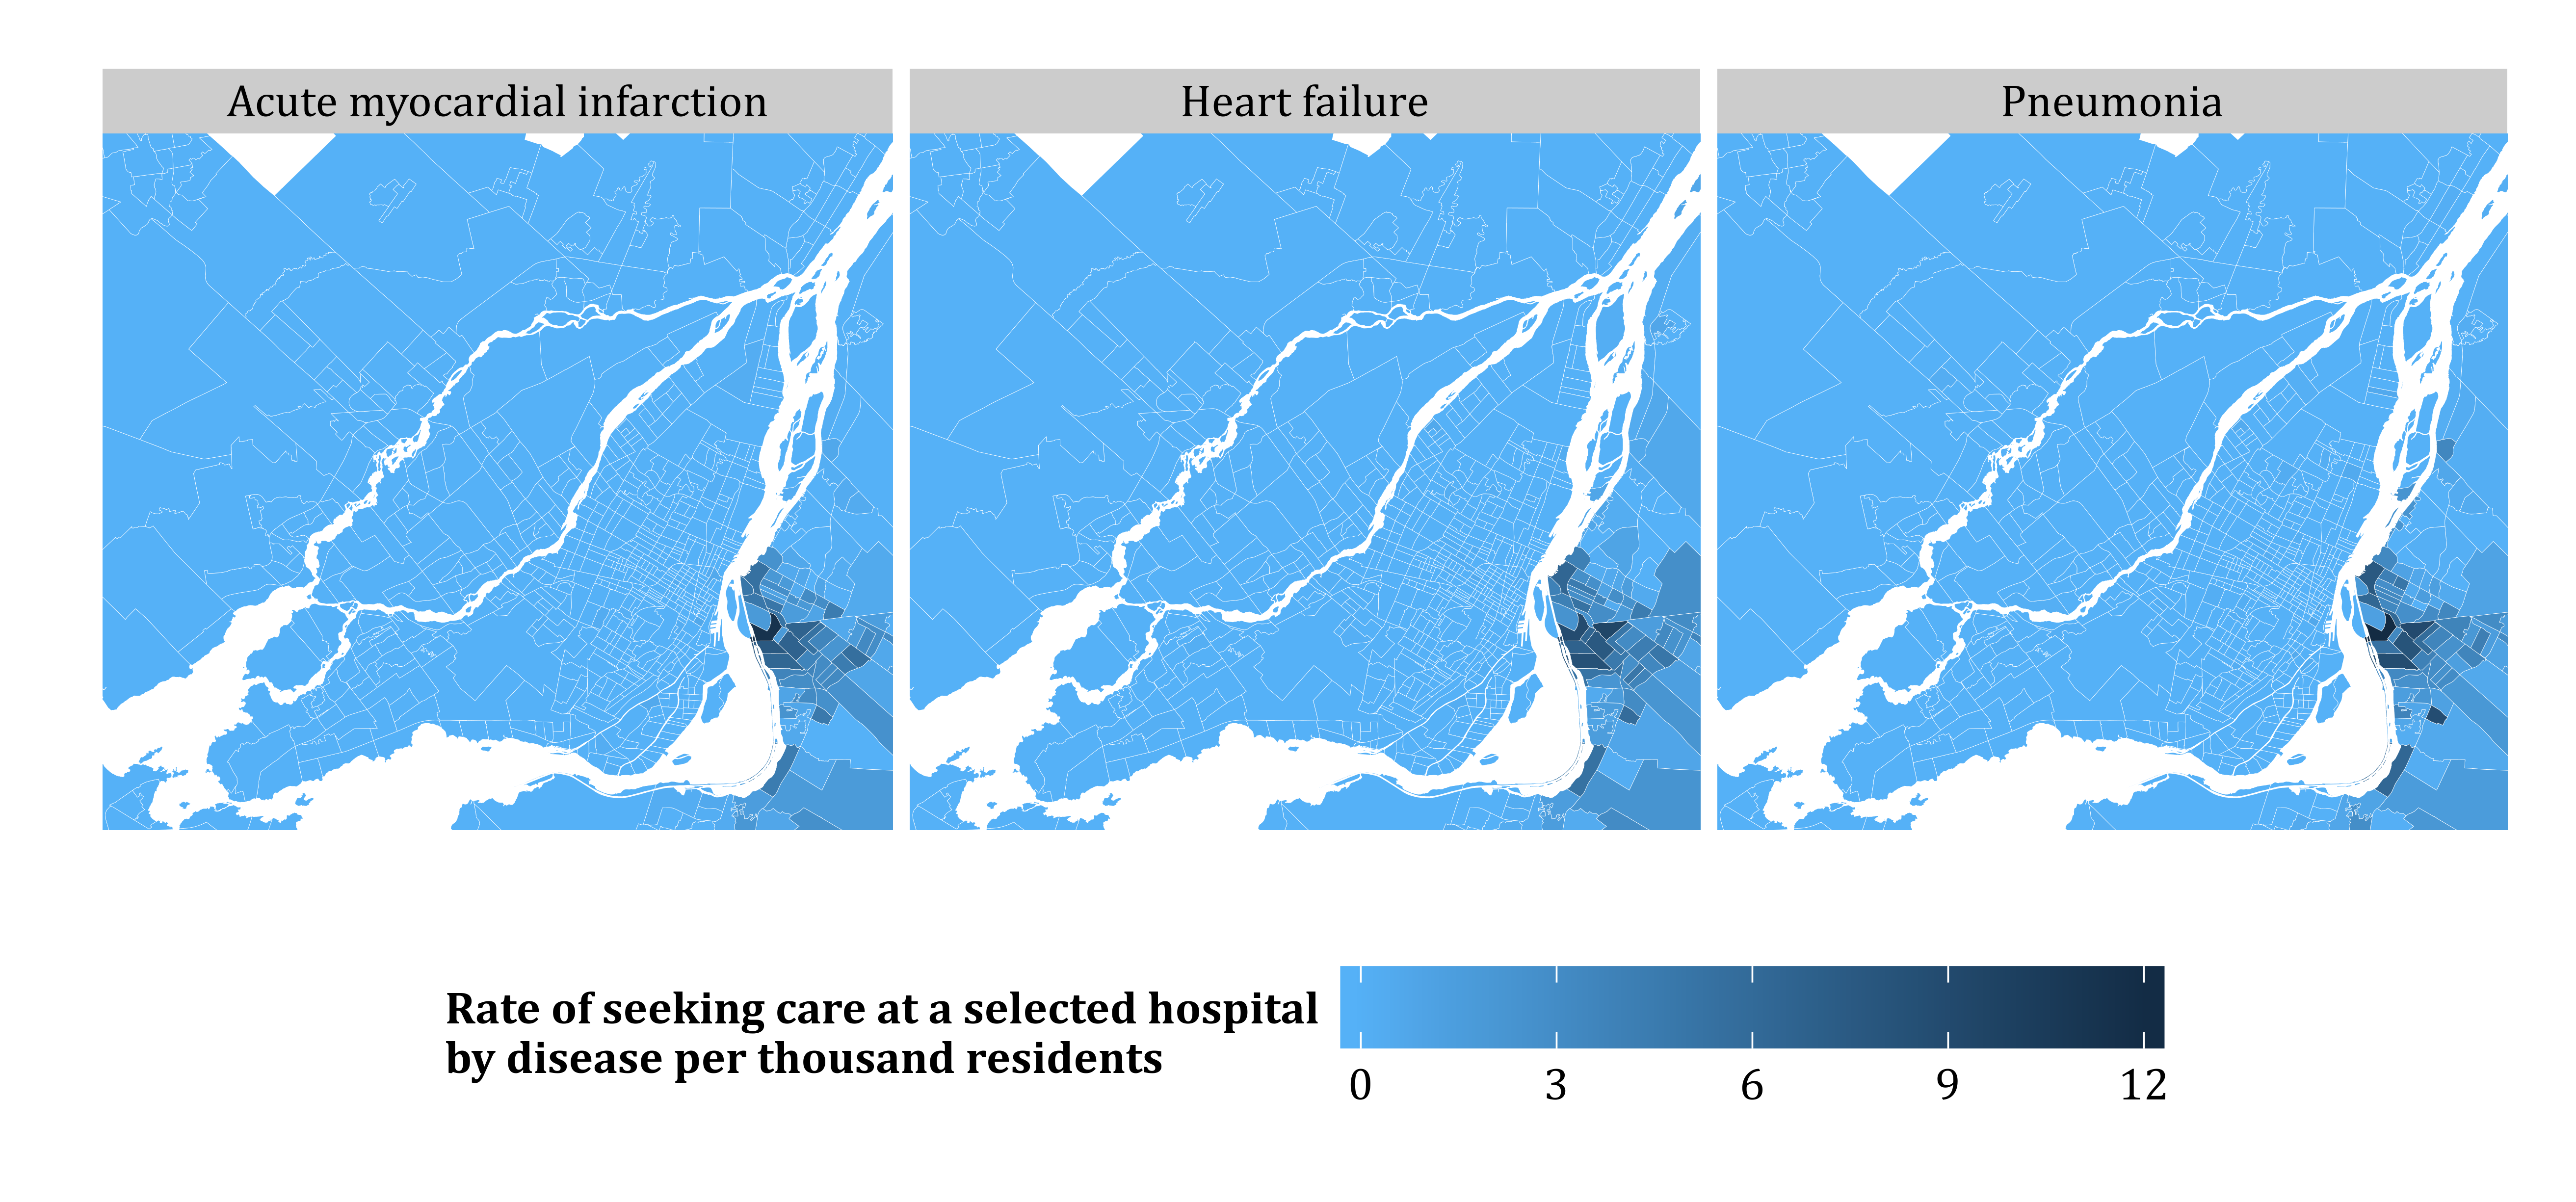
\includegraphics{../figures/hosp_choro.png}
    \caption[Rates of seeking care at a selected hospital by admission diagnosis.]
      {Rates of seeking care at a selected hospital by admission diagnosis. A descriptive sentence}
    \label{fig:hosp_choro}
\end{figure}

% What does the accuracy of the random forest model look like as the number of trees grows for both the Q model and the G model?
\begin{figure}[H]
    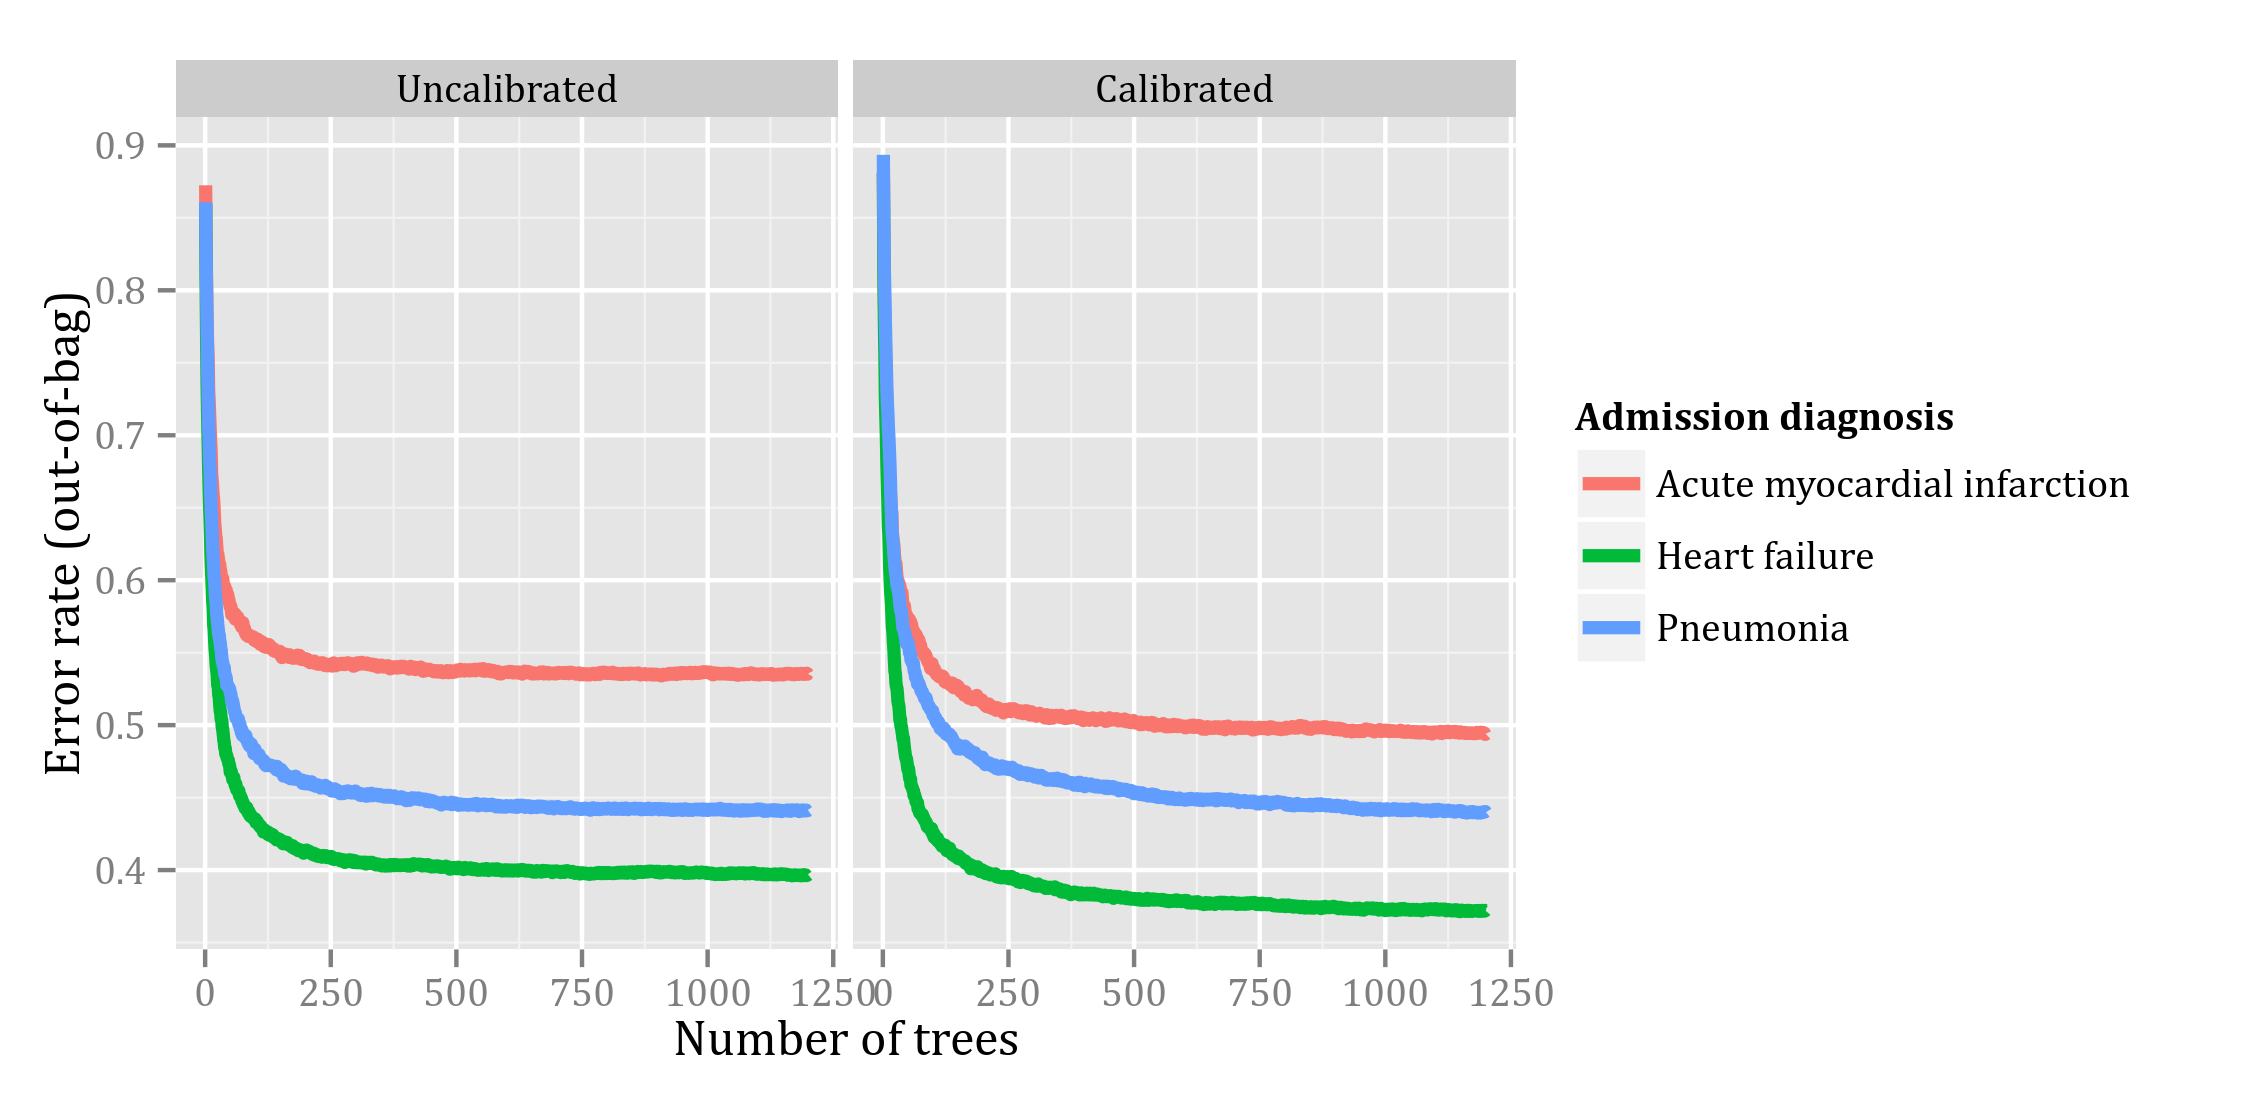
\includegraphics{../figures/error_rate_for_hospital_choice.png}
    \caption[Error rate for random forest model of hospital choice.]
      {Error rate for random forest model of hospital choice. A descriptive sentence.}
    \label{fig:error_rate_for_hospital_choice}
\end{figure}

% What are the top 10 predictive variables for the hospitals by disease?
\begin{figure}[H]
    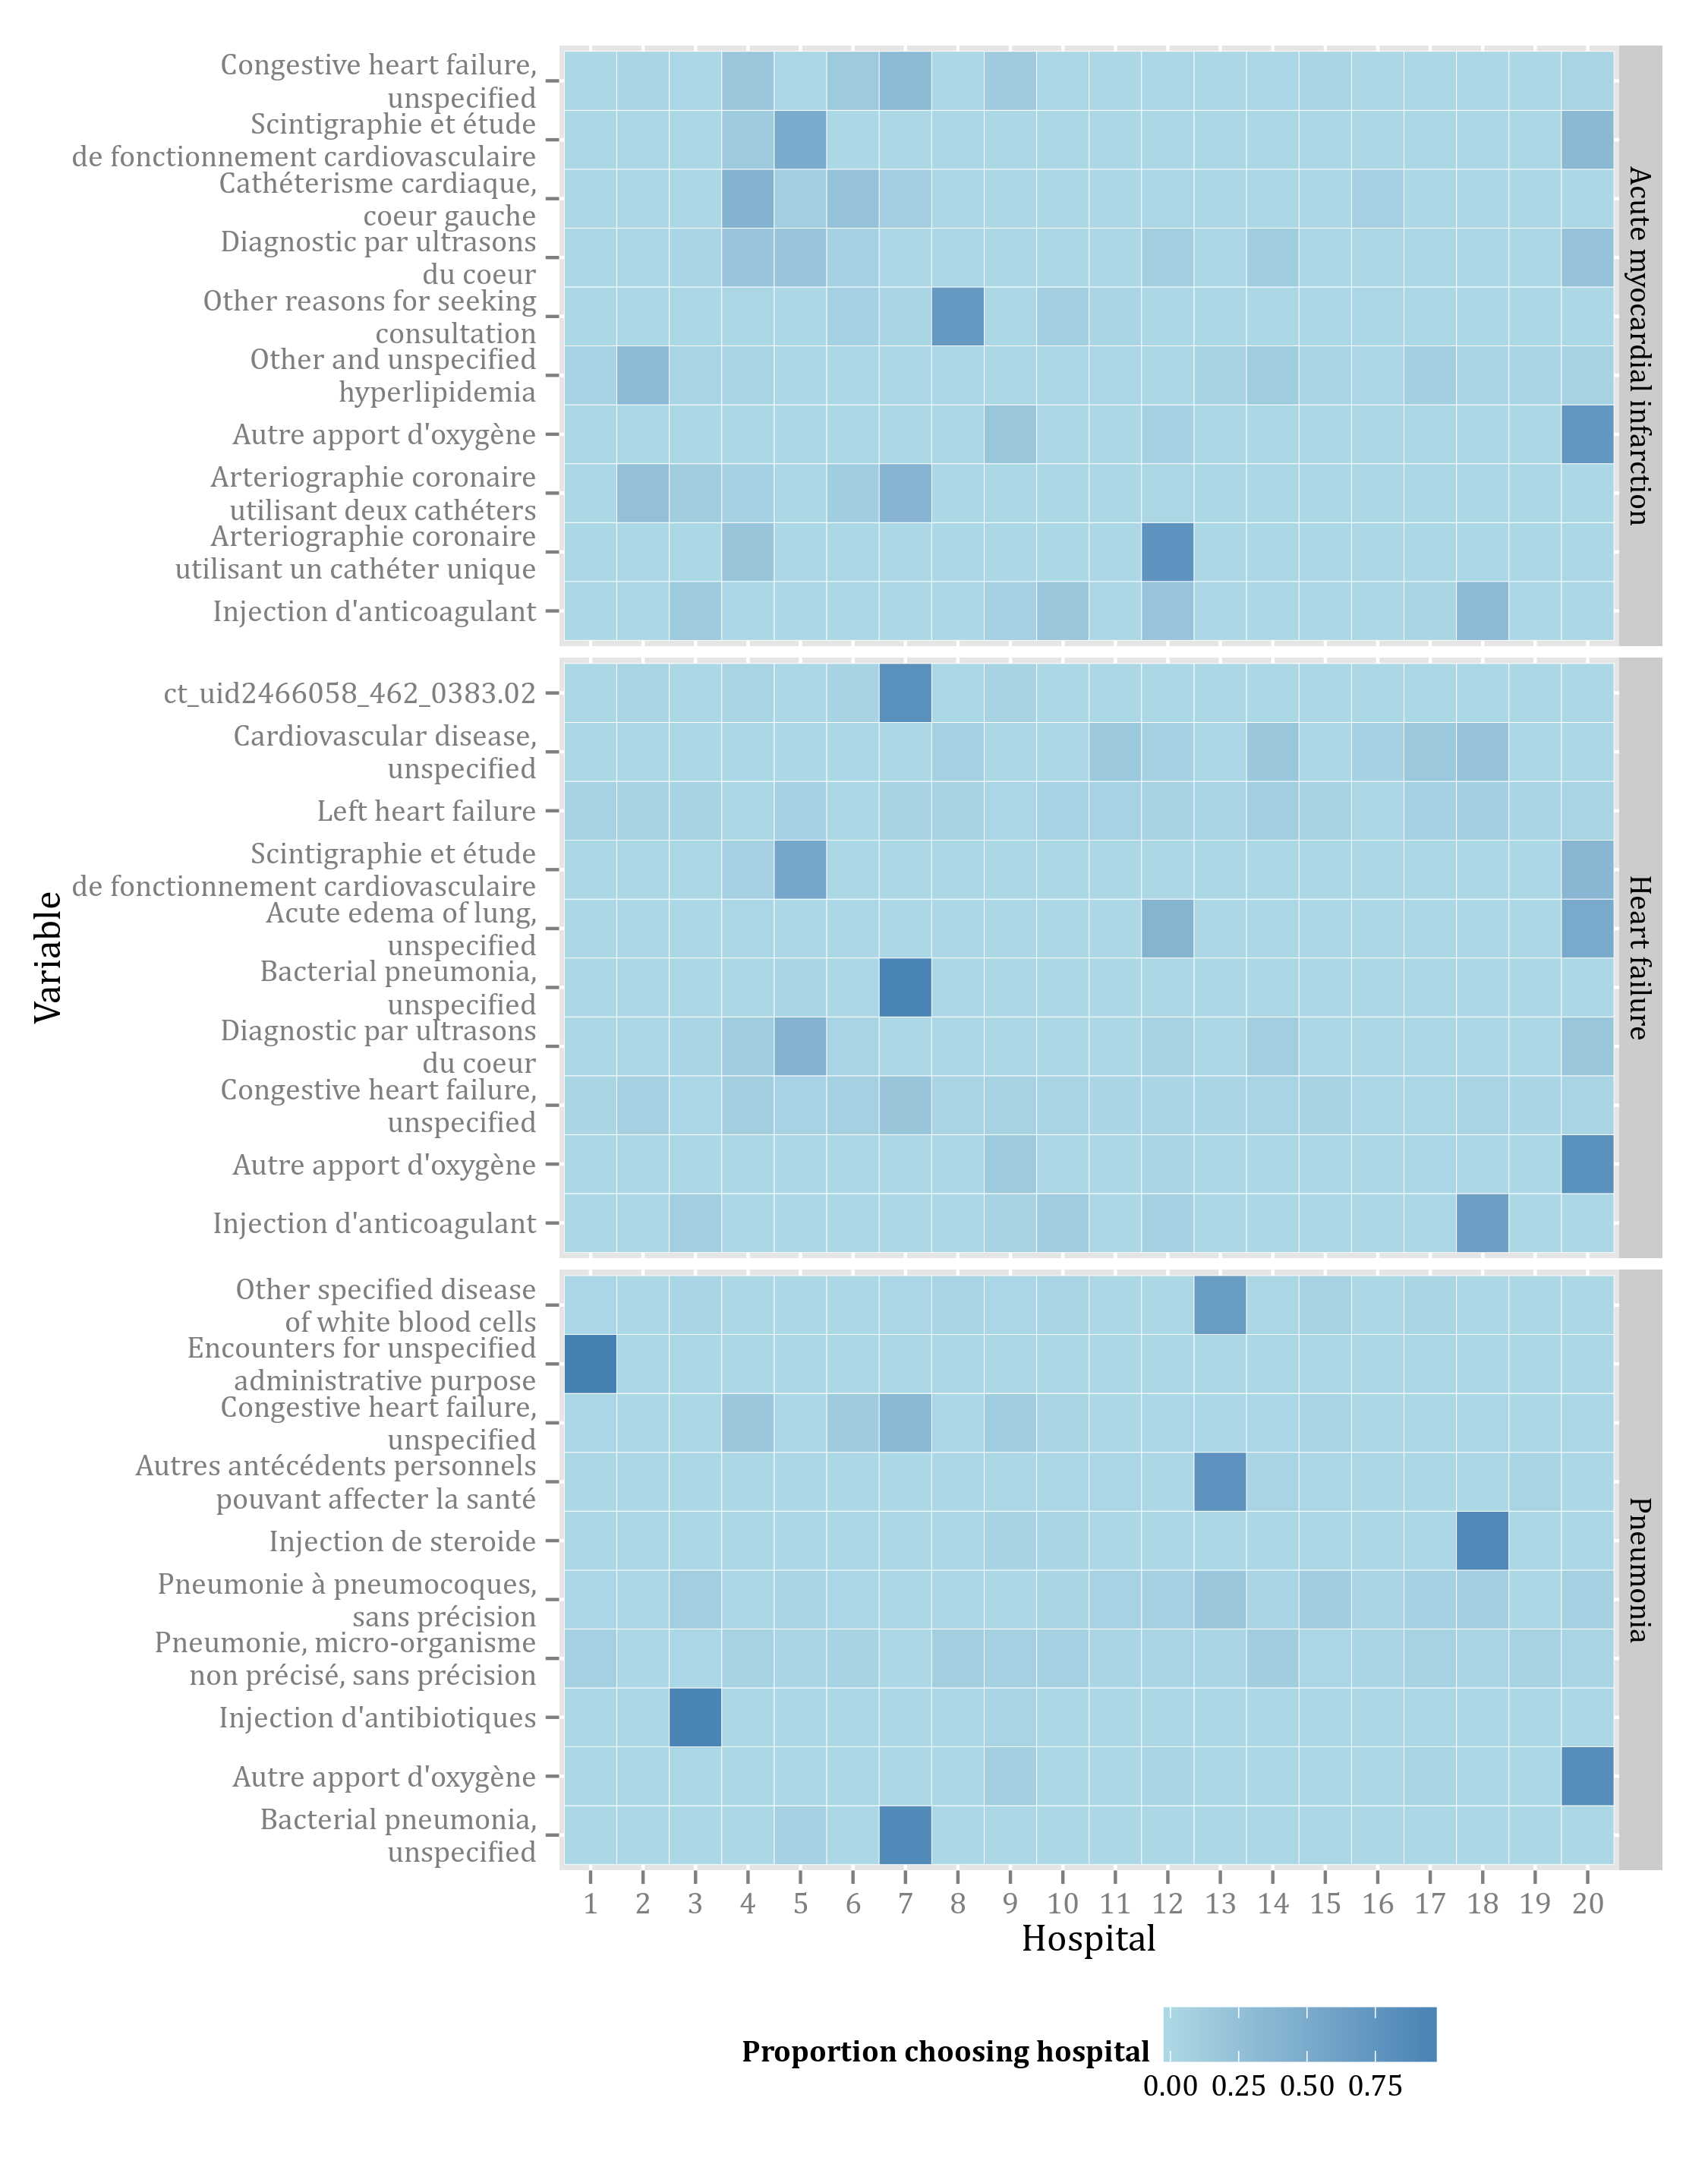
\includegraphics{../figures/top_10_variable_importance_and_hospital.png}
    \caption[Error rate for random forest model of hospital choice.]
      {10 most important variables for the G model, by disease. A descriptive sentence.}
    \label{fig:top_10_variable_importance_and_hospital}
\end{figure}

% How important are the different variables for each model by class?
\begin{figure}[H]
    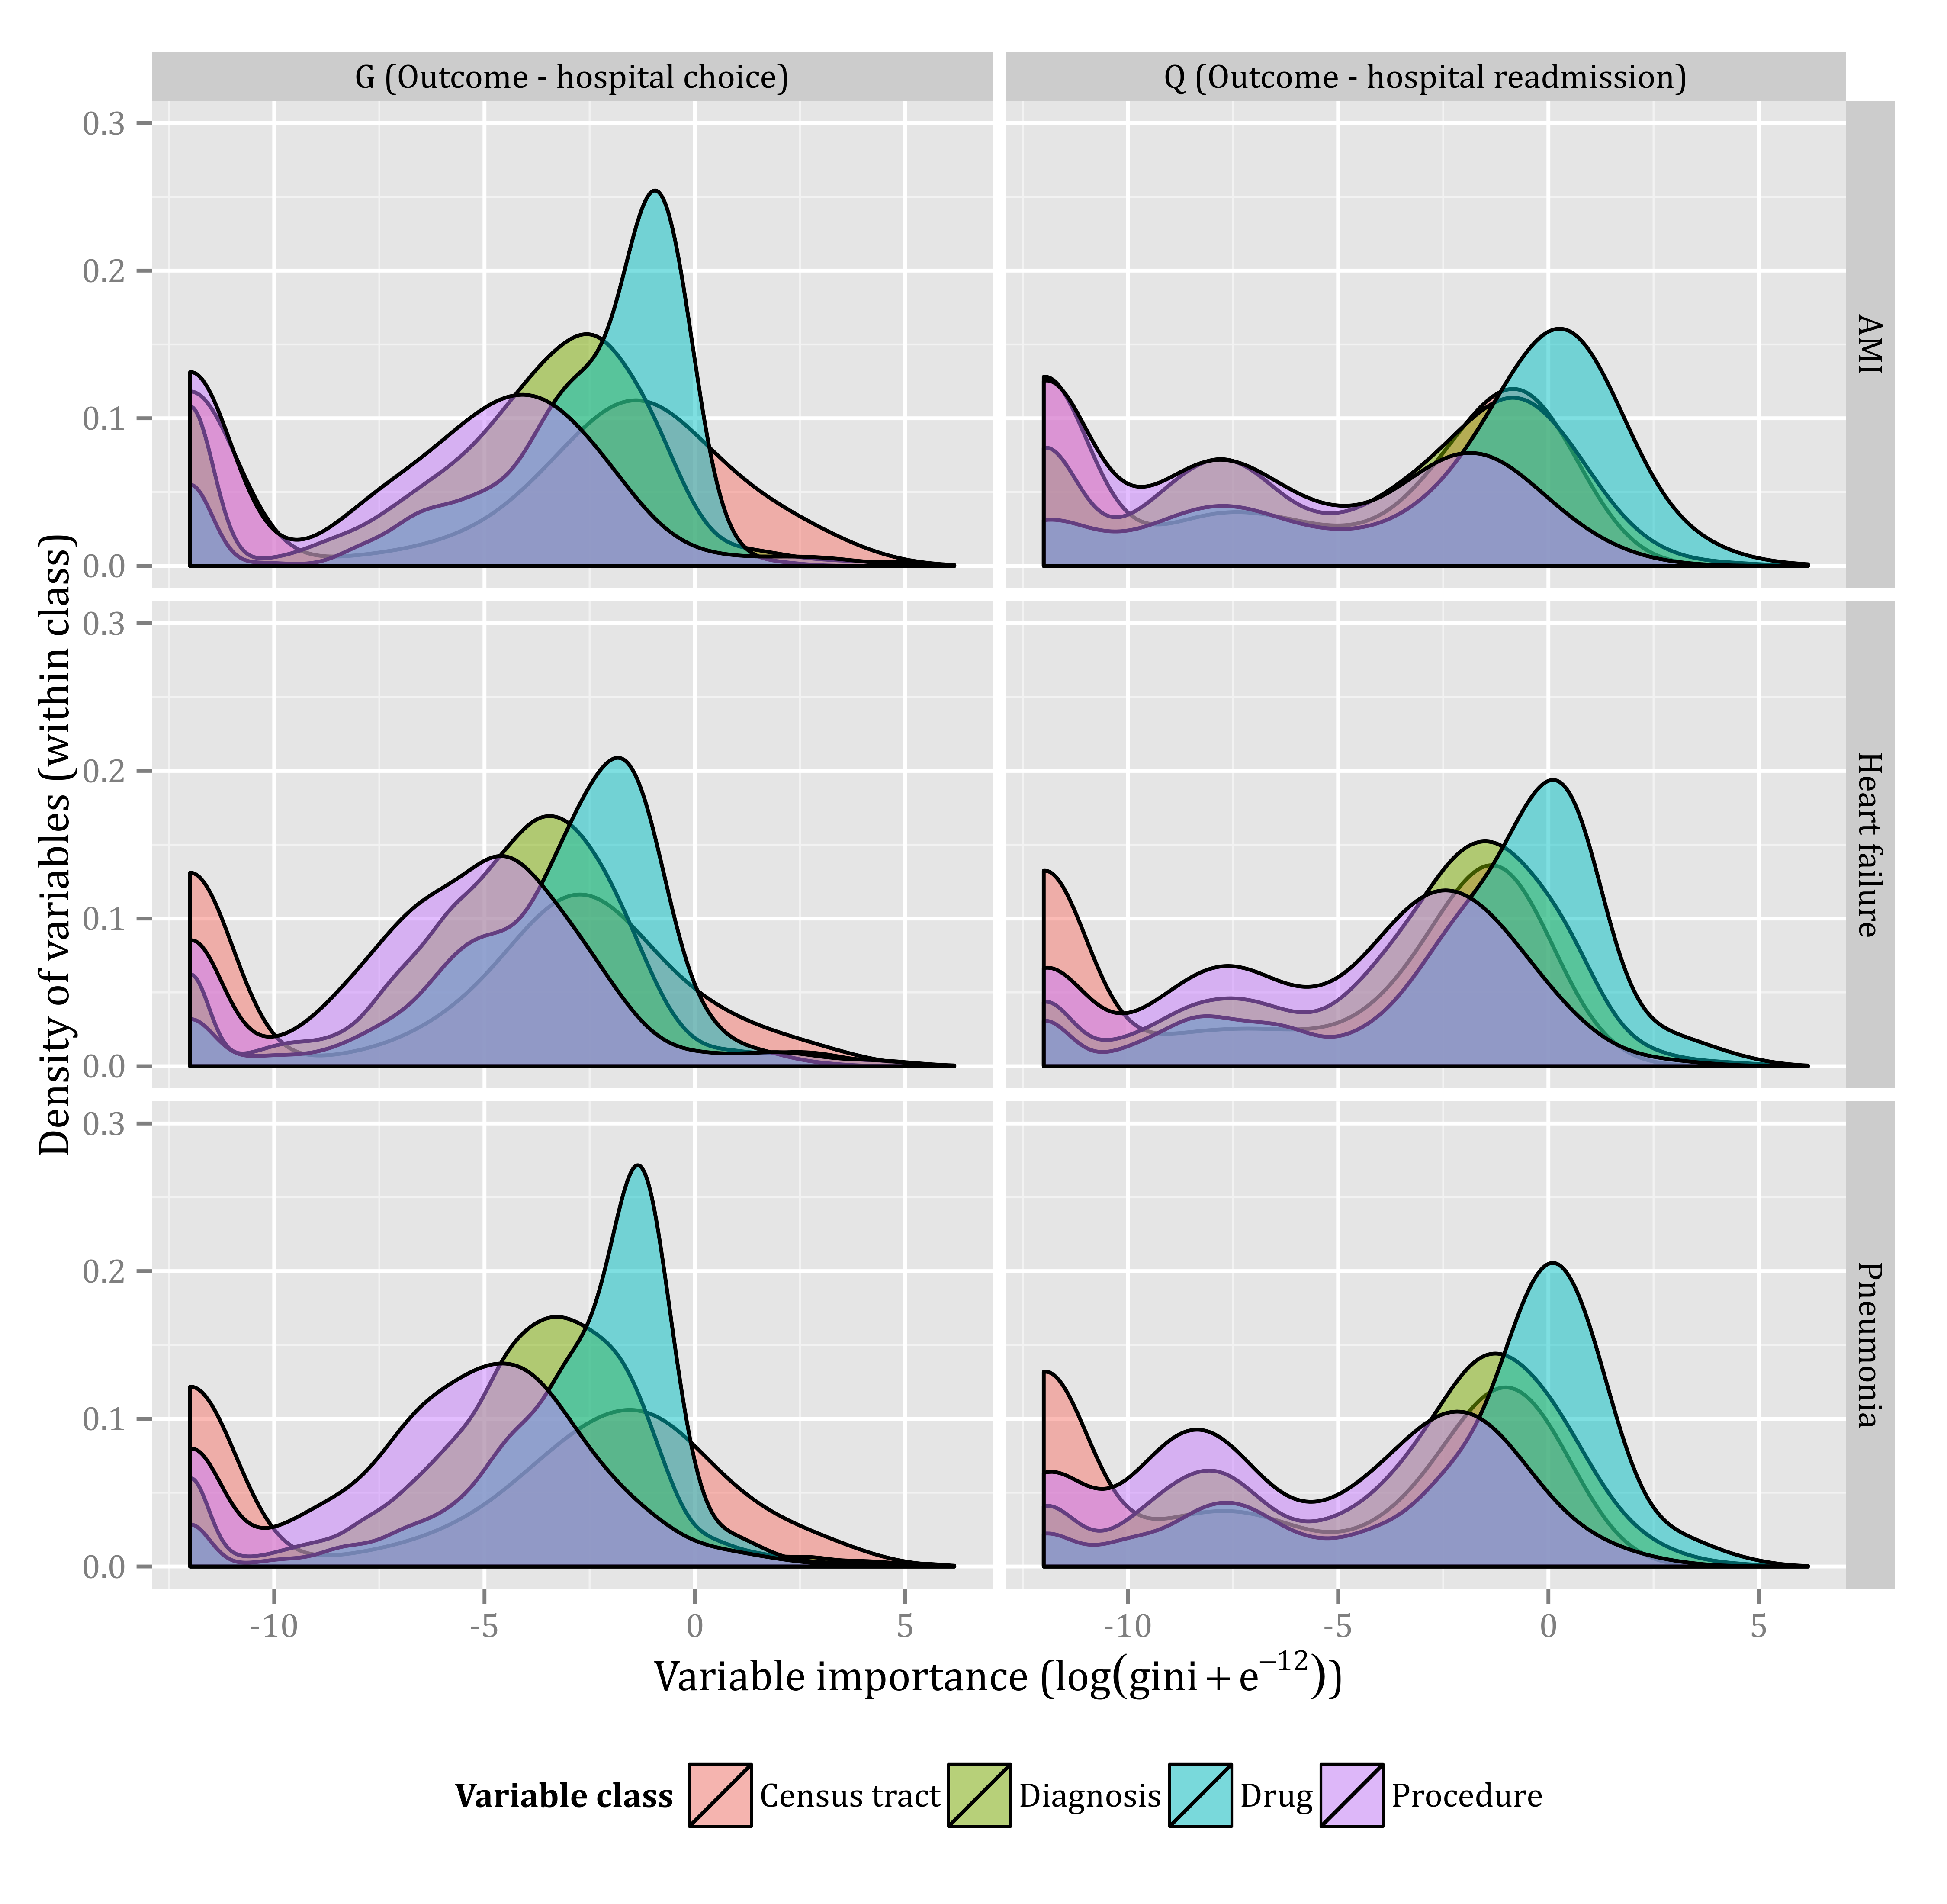
\includegraphics{../figures/variable_importance_by_model_and_class.png}
    \caption[Error rate for random forest model of hospital choice.]
      {Variable importance by model and variable class. A descriptive sentence.}
    \label{fig:variable_importance_by_model_and_class}
\end{figure}

% How does the glmnet model compare accuracy to the random forest model?
% What are the most important variables?

\section{Discussion}

\printbibliography

\end{document}
